\documentclass[landscape]{article}
\usepackage{tikz, siunitx}
\DeclareSIUnit{\solarmass}{\ensuremath{\mathrm{M_\odot}}}
\begin{document}
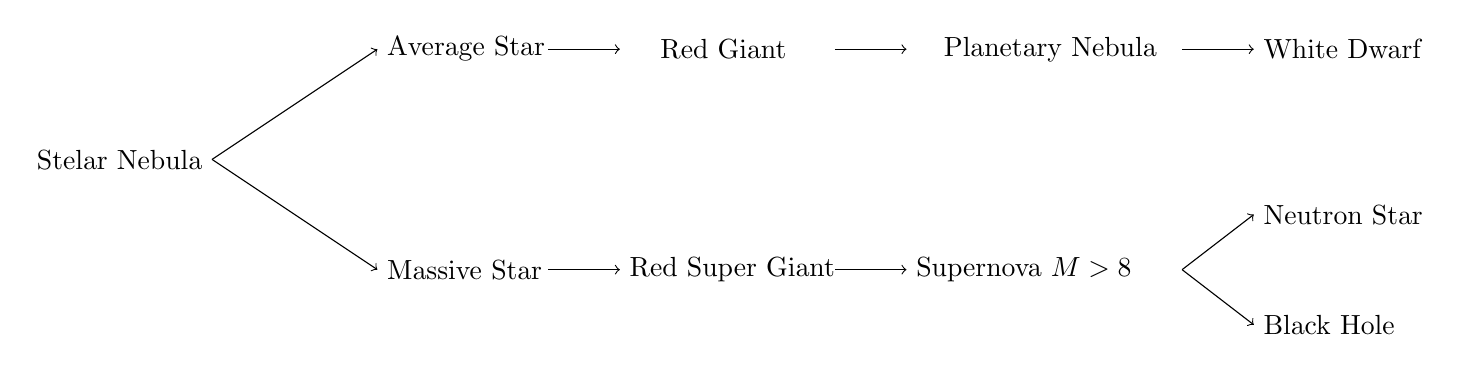
\begin{tikzpicture}[scale=0.7]
%\draw [ultra thin, lightgray] (0,0) grid (20,10);
\node [left] at (0,5) {Stelar Nebula};
\draw [->] (0,5) -- (3,7);
\draw [->] (0,5) -- (3,3);
\node [right] at (3,7) {Average Star};
\node [right] at (3,3) {Massive Star};
\begin{scope}[xshift=0.9cm]
\draw [->] (5.2,7) -- (6.5,7);
\draw [->] (5.2,3) -- (6.5,3);
\node [right] at (6.5,7) {\hphantom{Su}Red Giant\hphantom{per}};
\node [right] at (6.5,3) {Red Super Giant};
\begin{scope}[xshift=1.2cm]
\draw [->] (9.2,7) -- (10.5,7);
\draw [->] (9.2,3) -- (10.5,3);
\node [right] at (10.5,7) {\hphantom{\(88\)}Planetary Nebula};
\node [right] at (10.5,3) {Supernova \(M>\SI{8}{\solarmass}\)};
\begin{scope}[xshift=1.5cm]
\draw [->] (14,7) -- (15.3,7);
\draw [->] (14,3) -- (15.3,4);
\draw [->] (14,3) -- (15.3,2);
\node [right] at (15.3,7) {White Dwarf};
\node [right] at (15.3,4) {Neutron Star};
\node [right] at (15.3,2) {Black Hole};
\end{scope}
\end{scope}
\end{scope}
\end{tikzpicture}

\end{document}